\documentclass[letter,12pt]{article}
%\usepackage[doublespacing]{setspace}
\usepackage[margin=1in]{geometry}
\usepackage{natbib}
\usepackage{graphicx}
\usepackage{float}
\usepackage{amsmath}
\usepackage[super]{nth}
\usepackage[short]{optidef}
\usepackage{physics}
\usepackage{listings}
\usepackage{array}
\usepackage{hyperref}
\usepackage[justification=centering]{caption}
\lstset{breaklines=true}
\author{}
\title{}
\date{}
\usepackage{fancyhdr}
\pagestyle{fancy}
\lhead{14.03/14.003 Recitation 10}
\chead{}
\rhead{Jonathan Cohen (jpcohen@mit.edu)}
\lfoot{}
\cfoot{}
\rfoot{Page \thepage}



\begin{document}

\section{Overview of ``Lemons" Market Unraveling}

Analysis of markets with asymmetric information can be intimidating, but a lot of the intuition from standard markets carries through. The main distinction is that each side cares only about the good or service they buy/sell in standard markets, not the identity of the buyer or selling with whom they transact. This changes with asymmetric information, since one side can't actually observe the type of good or service they're buying/selling. Therefore they need to use information about the buyer/seller to infer the quality of the good or service.

Market unraveling broadly describes when mutually advantageous trades are unable to be realized due to asymmetric information. In the market for lemons, the setup is that sellers know quality while buyers do not.

\textbf{Key steps to understand how markets unravel}: Before listing for sale, what information does a seller have? For a given item listed for sale, what information does a buyer have? How does a seller take then take this into account?

Let's go through a mathematical example to formalize these ideas in a (hopefully) less convoluted way than the lecture notes.

\begin{itemize}
	\item Quality of good $\theta$ uniformly distributed on $[0,\bar{\theta}]$ observed only by seller
	\item Buyer utility $\theta-p$
	\item Seller utility $p-r(\theta)$
	\item Competitive equilibrium is single price (why?) $p^*$ s.t. all sellers value good less than $p^*$ and buyers expect to receive $p^*$ quality good
\end{itemize}

\textbf{Formal equilibrium conditions}:
\begin{align}
& \Theta^* = \{\theta : r(\theta)\leq p^* \} \text{(i.e. types of goods sold in equilibrium)}\\
& p^* = E[\theta | \theta \in \Theta^* \text{(i.e. equilibrium price given types of goods sold in equilibrium)}]
\end{align}

\subsection{Graphical analysis}:

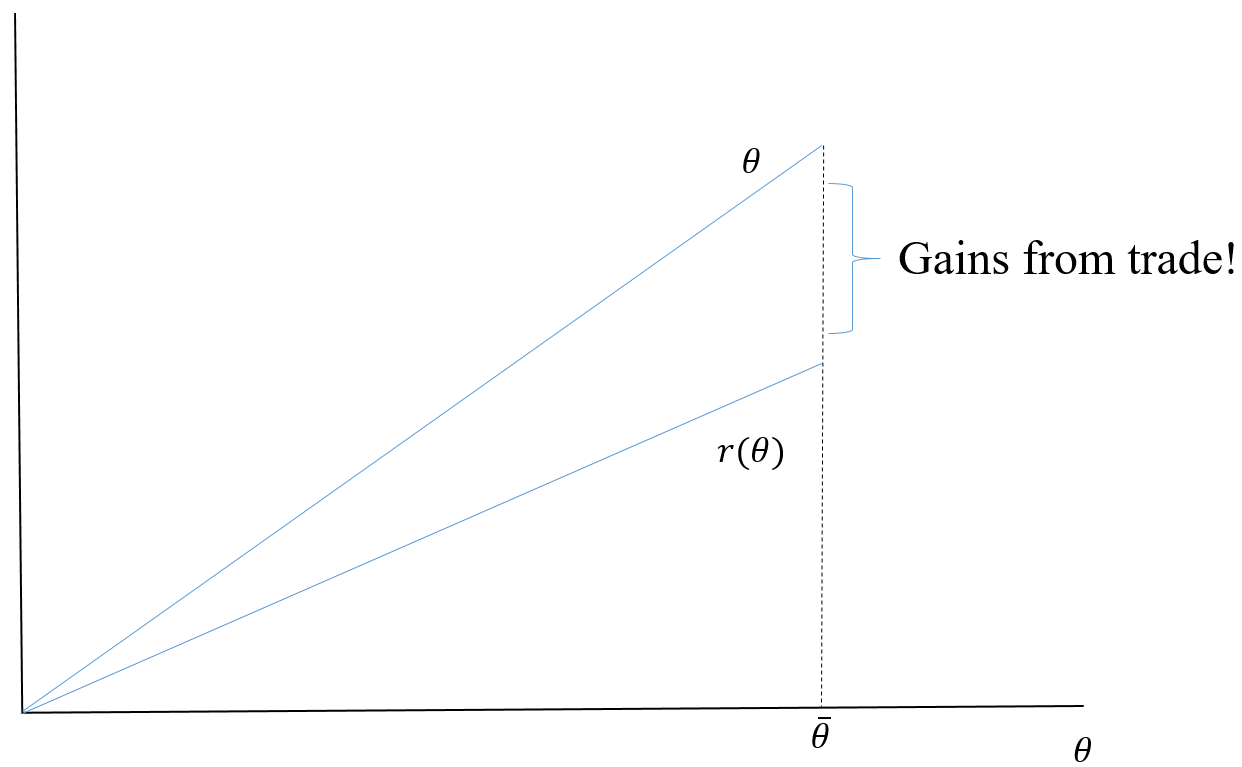
\includegraphics[width=.5\textwidth]{akerlof-setup.png}
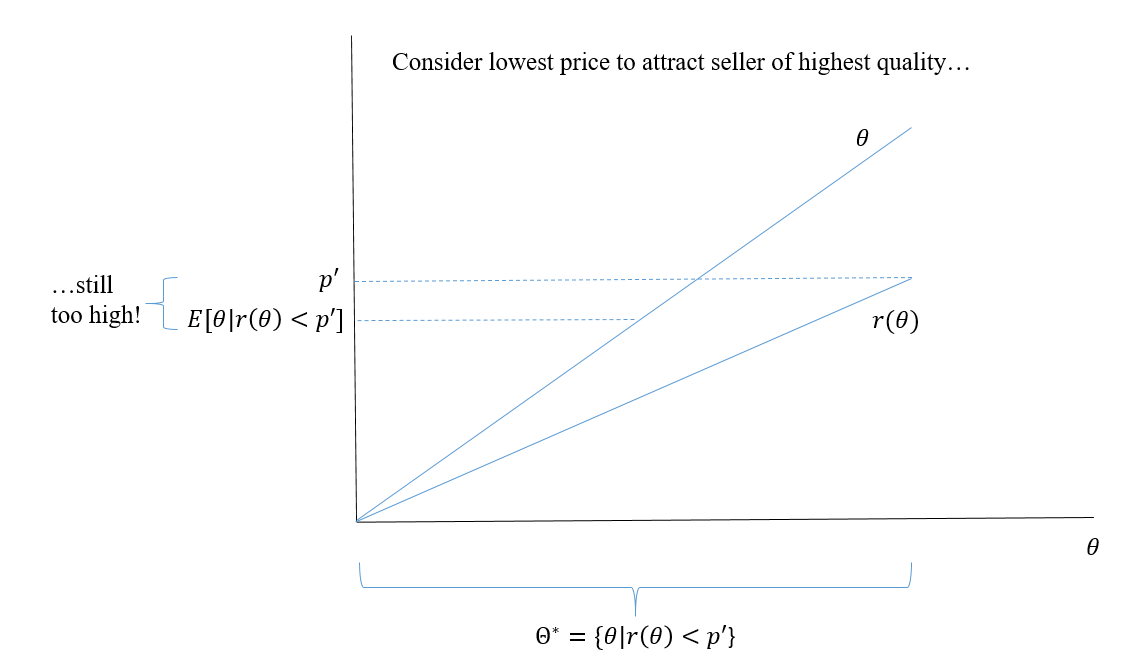
\includegraphics[width=.5\textwidth]{akerlof-start.png}

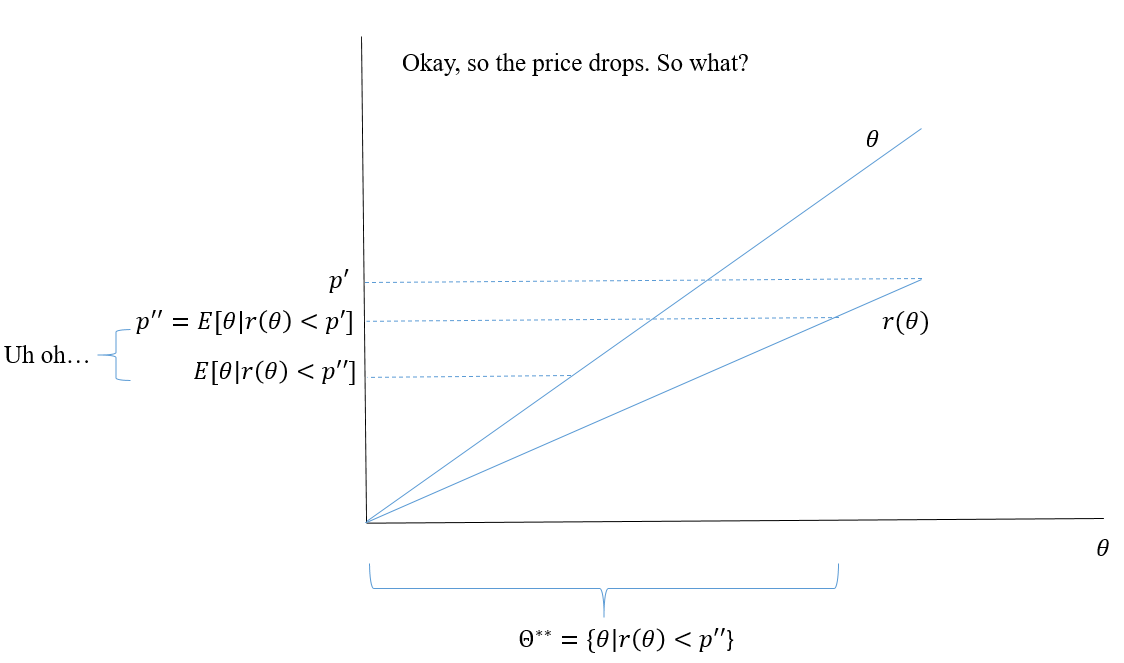
\includegraphics[width=.5\textwidth]{akerlof-so_on.png}
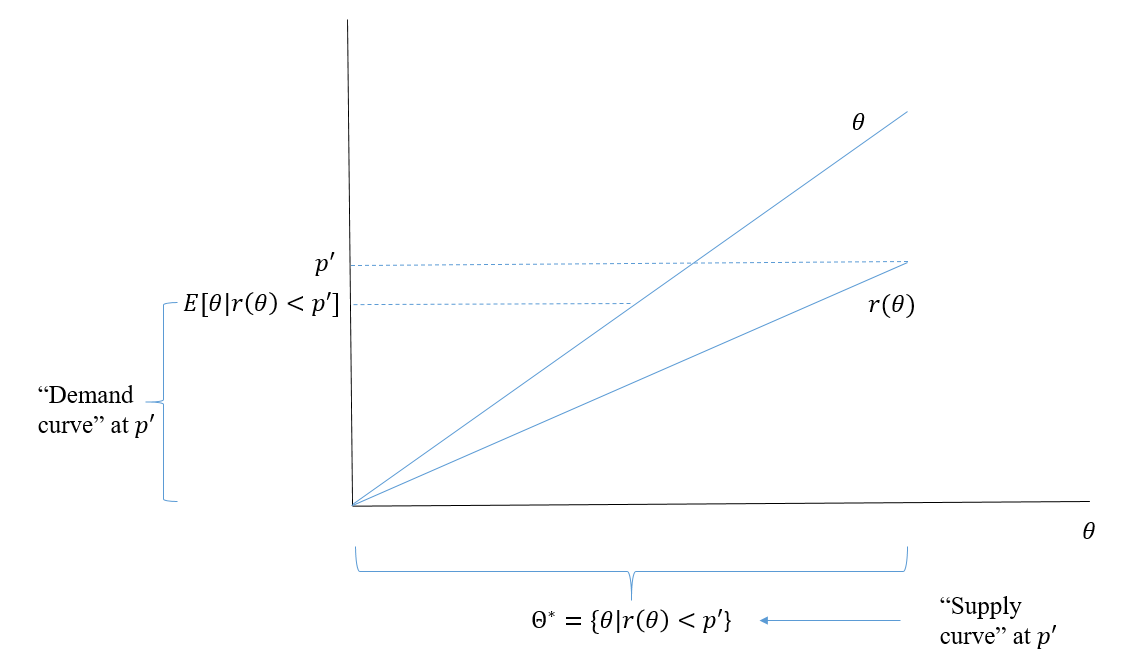
\includegraphics[width=.5\textwidth]{akerlof-SD.png}

Start with the upper-left graph. The 45 degree line $\theta$ represents buyer valuations, while the lower line $r(\theta)$ represents sellers' valuations (i.e. ``reservation" price). That sellers value the good less than buyers implies gains from trade. However, asymmetric information implies buyers know only the \textit{average} quality of goods transacted. 

The upper-right graph considers whether there could be an equilibrium with all goods sold. The lowest possible price of such an equilibrium is $p^*$ (i.e. $r(\bar{\theta})$). However, it turns out that the average valuation of buyers is less than $p^*$, so the price cannot be that high. 

The lower-left graph considers a different equilibrium where the price is lowered. This leads to some sellers dropping out of the market, which in turn lowers the average valuation of buyers. You can imagine many of these graphs showing the complete unraveling of the market.

The lower-right graph presents alternate intuition about each stage. For a given price, the number of sellers willing to transact is ``supply", while the number of buyers willing to transact is ``demand". The equilibrium condition then looks a lot like standard market analysis where we require ``demand" = ``supply".

\subsection{Mathematical analysis}:

Suppose $\theta \sim U[0,1]$ and $r(\theta)=\frac{2}{3}\theta$. Then for a proposed equilibrium $p^*$, buyer willingness to pay is: $$E[\theta|r(\theta)\leq p^*]$$ Substituting the expression for $r(\theta)$: $$E[\theta|\frac{2}{3}\theta\leq p^*]$$ Rearranging to make this in the familiar form for expectations: $$E[\theta|\theta\leq \frac{3}{2}p^*]$$ 

It should be clear that uniformly distributed quality means that the average transacted good's quality will be half of the equilibrium price. Moreover, since the highest quality good is 1, this must be at most 1/2. Therefore, the above expression for willingness to pay is: $$\min\{\frac{3}{4}p^*,\frac{1}{2} \}$$.

The equilibrium therefore requires $p^*=\min\{\frac{3}{4}p^*,\frac{1}{2} \}$, which is uniquely satisfied by $p^*=0$ (i.e. complete unraveling).

\subsection{Additional adverse selection practice problem}

In the market for used cars, there are high and low quality cars. At a price $P$, the quantity of high and low quality cars supplied are (in thousands of cars): $\max(2P -8, 0)$ and $\max(P - 3, 0)$ respectively. To buyers, a low quality car is worth 4.5 and a high quality car is worth 7. Buyers are risk neutral, and if they are uncertain about the quality of the car, their valuation is the expected value given their beliefs about the quality. The number of buyers far exceeds the number of sellers, so the demand for cars is infinite if the price is less than the expected value of a car.

\begin{enumerate}
	\item Suppose that buyers are perfectly informed about the quality of each car. What is the market price
	and quantity of high and low quality cars? You may find it helpful to graph the supply and demand
	curves.
	\item Suppose now that buyers have no information about what kind of car they are purchasing. If the
	prevailing market price for cars is $P$, what fraction of the cars available for sale are high quality? At
	that price $P$, what are the buyers’ expected valuation for the cars?
	\item There is some price $P$ such that the buyer’s willingness to pay for a car is equal to price $P$. What is the
	quantity of high and low quality cars traded in this equilibrium? Make sure these answers are intuitive.
	\item Now suppose instead that the supply for high quality cars was $2P - 11$. If you were to solve part 3,
	you would find that there is no real solution to the quadratic function. What is the equilibrium in this
	market? Why does the solution change so much?
\end{enumerate}


\section{Overview of Signaling Models}

The above analysis related to market unraveling relied on one side of the market needing to make an inference about the other due to asymmetric information. In some sense, this was all passive based on willing to participate in the market or not; all market participants get pooled together. It makes sense that market participants might want to actively convey information to the other side to facilitate trade. This is the heart of signaling models.

Nonetheless, the analytical tools turn out to be the same: given a proposed equilibrium, you (1) deduce what one side of the market infers about the other and then (2) consider whether that's consistent with the proposed equilibrium.


\subsection{Problem Set 6 intuition}

The problem set makes this slightly more concrete by considering the case of job market signaling. In the absence of a skills test, high and low ability programmers are \textit{pooled} together. Because programmers are paid according to their \textit{expected} ability, high ability programmers are underpaid while low overpaid. This generates an obvious incentive for high ability programmers to differentiate themselves.

The basic analytic strategy is as follow:
\begin{enumerate}
	\item Consider a given equilibrium (e.g. pooling vs. separating)
	\item Specify the actions associated with that equilibrium (e.g. everybody passing the test with pooling vs. only high ability passing the test with separating)
	\item Consider what each side infers about the other with that equilibrium (e.g. population average ability with pooling vs. exact ability with separating)
	\item Consider payoffs associated with those actions and inferences (e.g. costs of passing the test or not vs. benefits of wage)
	\item Check whether either type has an incentive to deviate (e.g. break a pooling equilibrium by the low type choosing to forgo passing the test and revealing themselves as low type)
\end{enumerate}


\subsection{Additional signaling practice problem}

%source: https://www.ssc.wisc.edu/~mweretka/301_15/PS/PS12.pdf

Suppose I'm looking for someone to do data analysis as a UROP. The pool of undergrads consists evenly (i.e. 50\%/50\%) of two types: workaholics $(w)$ and lazybones $(l)$. The productivity of a workaholic is 10 regressions/day, while a lazybone produces only 4/day. Each regression gets me a \$1 larger stipend (I wish!), and Tobias mandates that I pay my UROP's their expected productivity.

\begin{enumerate}
	\item What's the wage in a pooling equilibrium?
	\item Andrea has offered to screen UROP's on my behalf. He administers a test that costs \$1 to take, and he allows potential UROP's to take it multiple times. He's sneaky, so he keeps the profits and tells me only how many tests the potential UROP passed. Workaholics are studious, so they can always pass Andrea's test. Lazybones slack off, so it always takes them two attempts to achieve one passed test.

	Question: Are two passed tests a credible signal that a worker is a workaholic? Why or why not?
	\item What is the minimal number of tests that constitutes a credible signal of being a workaholic for the employer?
	\item Is signaling in the form of taking tests efficient from the point of view of society?
\end{enumerate}


\section{Solutions}

\begin{itemize}
	\item Adverse selection problem
	\begin{enumerate}
		\item In the market for low quality cars, supply is $P-3$ and consumers will purchases if $P\leq4.5$. The equilibrium price is $P=4.5$, with $Q=1.5$.
		
		In the market for high quality cars, supply is $2P-8$ and consumers are willing to pay 7. The equilibrium price is $P=7$, with $Q=6$.
		
		Prices won't be higher than these because then demand goes to 0. Prices will not be lowers because demand for cars is perfectly elastic.
		
		\item At price $P$, there are $2P-8$ high quality cars and $P-3$ low quality cars, for a total of $3P-11$ cars. To the buyer, any unknown car is high quality with probability $(2P-8)/(3P-11)$ (note the car is low probability with complementary probability $1-(2P-8)/(3P-11)=(P-3)/(3P-11)$).
		
		If the buyer believes a car to be high quality with probability $\lambda$, his valuation is $7\lambda - 4.5(1-\lambda)$. In this case, the probability is what we calculated above, and his expected value is $7*(2P-8)/(3P-11)+4.5*(P-3)/(3P-11)$.
		
		\item We are looking for some price $P$ such that the market price leads buyers to be the same as the buyer's expected value (since demand is perfectly elastic). That is, we are looking to solve: $7*(2P-8)/(3P-11)+4.5*(P-3)/(3P-11)=P$. Tedious algebra (or WolframAlpha) gives a quadratic with two solutions: $P=5.92$ and $P=3.90$. Note that at the latter price no high quality cars are sold (due to the high quality car supply curve $Q^S_H=2P-8$)
		
		
	\end{enumerate}
	\item Signaling problem
	\begin{enumerate}
		\item 7 (Wage in competitive pooling equilibrium is expected productivity)
		\item Two passed tests is not a credible signal. This is because in the separating equilibrium,
		the additional benefit from being known as a workaholic as opposed to a lazybones is $w^W-w^L = 10 − 4 = 6$
		
		Since to pass two tests, it costs the lazybones only $c^L(2)=2*2-4$, so the lazybones take the tests (as do the workaholics).
		\item The minimum credible number of passed tests is the one that just prevents the lazybones from taking the tests (and obtaining wage $w^W$ instead of $w^L$). It is the $e$ such that $c^L(e)\geq6$, so $c^L(e)\geq 6 \Rightarrow 2e\geq 6 \Rightarrow e\geq 3$.
		
		So $e = 3$ is a sufficient number of tests to lead to a separating equilibrium. (Assuming that at $e = 3$, the lazybones will not take the tests as he is indifferent at that point, so we can assume only the workaholics are the ones taking the tests. Note that the highest number of tests the workaholic would take anyway is 6.)

		\item In a separating equilibrium, the workaholics will be forced to take three tests. Because such tests do not improve the productivity of the workers, the tests are a waste of resources and Pareto inefficient. (However this is inefficient only compared to a world with perfect information!)

	\end{enumerate}
\end{itemize} 


\section{Visualizing Causal Inference}

For visual learners, here are some gifs to understand the causal inference tools we've used throughout the course. The nice thing is that you can understand the methods on a more formal level without any additional math.

\begin{itemize}
	\item Twitter thread with series of gifs: 
	
	https://twitter.com/nickchk/status/1068215492458905600
	\item Website with detailed discussion of each type of tool, including analysis using directed acyclic graphs:
	
	http://www.nickchk.com/causalgraphs.html
\end{itemize}



\end{document}